\documentclass[tikz,border=2mm]{standalone}
\usetikzlibrary{positioning,arrows.meta,calc,decorations.pathreplacing,shapes.geometric,fit}
\begin{document}
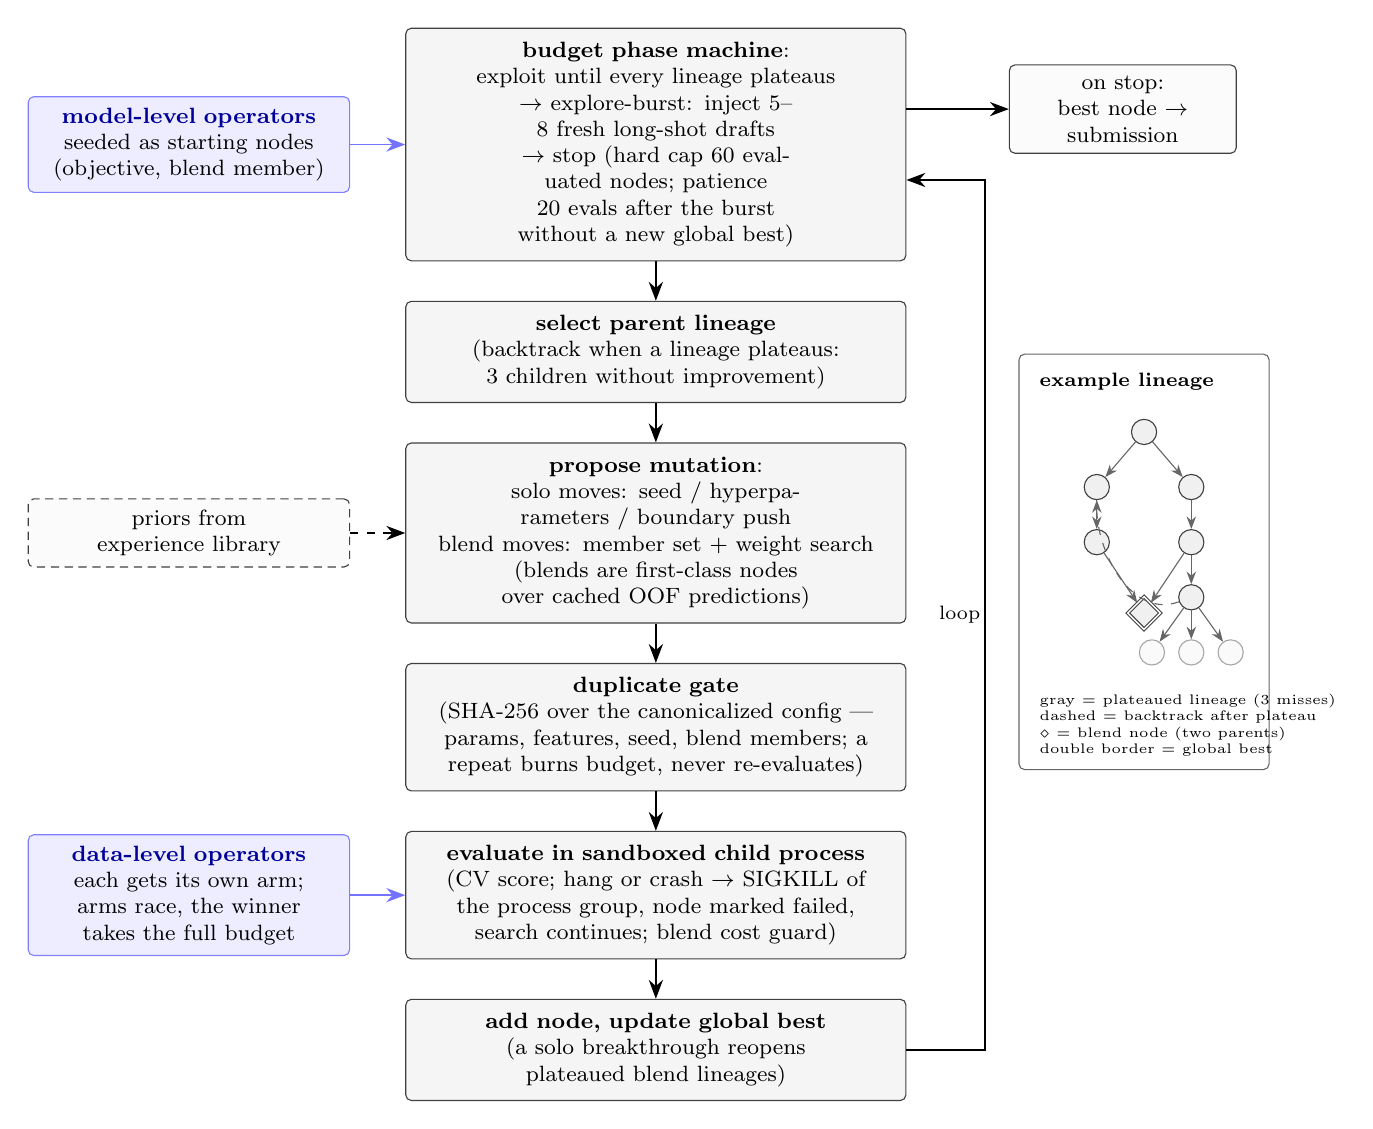
\begin{tikzpicture}[
  font=\footnotesize,
  sbox/.style={draw=black!75, rounded corners=2pt, align=center, inner sep=5pt,
               fill=gray!8, text width=60mm},
  sidebox/.style={draw=black!75, rounded corners=2pt, align=center, inner sep=4pt,
                  fill=gray!3, text width=38mm},
  injside/.style={sidebox, fill=blue!7, draw=blue!50},
  arr/.style={-{Stealth[length=2.4mm]}, semithick},
  barr/.style={arr, blue!55},
  darr/.style={arr, dashed},
  lab/.style={font=\scriptsize, inner sep=1.5pt},
  node distance=5mm
]
% ----- main loop column -----
\node[sbox] (phase) {\textbf{budget phase machine}:\\exploit until every lineage plateaus\\$\to$ explore-burst: inject 5--8 fresh long-shot drafts\\$\to$ stop (hard cap 60 evaluated nodes; patience\\20 evals after the burst without a new global best)};
\node[sbox, below=of phase] (select) {\textbf{select parent lineage}\\(backtrack when a lineage plateaus: 3 children without improvement)};
\node[sbox, below=of select] (propose) {\textbf{propose mutation}:\\solo moves: seed / hyperparameters / boundary push\\blend moves: member set + weight search\\(blends are first-class nodes over cached OOF predictions)};
\node[sbox, below=of propose] (dedup) {\textbf{duplicate gate}\\(SHA-256 over the canonicalized config --- params, features, seed, blend members; a repeat burns budget, never re-evaluates)};
\node[sbox, below=of dedup] (eval) {\textbf{evaluate in sandboxed child process}\\(CV score; hang or crash $\to$ SIGKILL of the process group, node marked failed, search continues; blend cost guard)};
\node[sbox, below=of eval] (add) {\textbf{add node, update global best}\\(a solo breakthrough reopens plateaued blend lineages)};
\foreach \a/\b in {phase/select, select/propose, propose/dedup, dedup/eval, eval/add}{\draw[arr] (\a) -- (\b);}
% ----- loop back, right side -----
\draw[arr] (add.east) -- ++(10mm,0) |- node[lab, pos=0.25, left]{loop} ([yshift=-4.5mm]phase.east);
% ----- exit, top right -----
\node[sidebox, text width=26mm, anchor=west] (out) at ([xshift=13mm, yshift=4.5mm]phase.east)
  {on stop:\\best node $\to$ submission};
\draw[arr] ([yshift=4.5mm]phase.east) -- (out.west);
% ----- inset: example lineage (schematic) -----
\begin{scope}[shift={(5.35,-3.1)},
  tn/.style={circle, draw=black!75, fill=gray!12, inner sep=0pt, minimum size=3.2mm},
  pl/.style={tn, draw=black!35, fill=gray!4, text=black!40},
  bl/.style={tn, diamond, fill=gray!12, minimum size=4.2mm, inner sep=0pt},
  te/.style={-{Stealth[length=1.6mm]}, thin, black!60}]
  \node[draw=black!60, rounded corners=2pt, fit={(-0.65,0.35) (2.35,-4.75)},
        inner sep=2.5pt] (insetframe) {};
  \node[font=\scriptsize\bfseries, anchor=north west] at (-0.6,0.32) {example lineage};
  \node[tn] (r)  at (0.85,-0.55) {};
  \node[tn] (A)  at (0.25,-1.25) {};
  \node[tn] (B)  at (1.45,-1.25) {};
  \node[tn] (B1) at (1.45,-1.95) {};
  \node[tn] (B2) at (1.45,-2.65) {};
  \node[pl] (c1) at (0.95,-3.35) {};
  \node[pl] (c2) at (1.45,-3.35) {};
  \node[pl] (c3) at (1.95,-3.35) {};
  \node[tn] (A1) at (0.25,-1.95) {};
  \node[bl, double, double distance=0.5pt] (bd) at (0.85,-2.85) {};
  \foreach \a/\b in {r/A, r/B, B/B1, B1/B2, B2/c1, B2/c2, B2/c3, A/A1}{\draw[te] (\a) -- (\b);}
  \draw[te] (B1) -- (bd); \draw[te] (A1) -- (bd);
  \draw[te, dashed] (B2) to[out=200, in=-90] (A);
  \node[font=\tiny, anchor=north west, align=left] at (-0.6,-3.75)
    {gray = plateaued lineage (3 misses)\\dashed = backtrack after plateau\\$\diamond$ = blend node (two parents)\\double border = global best};
\end{scope}
% ----- side inputs, left column -----
\node[injside, left=7mm of phase] (injcfg)
  {\textcolor{blue!60!black}{\textbf{model-level operators}}\\seeded as starting nodes\\(objective, blend member)};
\draw[barr] (injcfg) -- (phase);
\node[sidebox, densely dashed, left=7mm of propose] (prior)
  {priors from\\experience library};
\draw[darr] (prior) -- (propose);
\node[injside, left=7mm of eval] (injdata)
  {\textcolor{blue!60!black}{\textbf{data-level operators}}\\each gets its own arm; arms race, the winner takes the full budget};
\draw[barr] (injdata) -- (eval);
\end{tikzpicture}
\end{document}
